% Generated by Sphinx.
\def\sphinxdocclass{report}
\documentclass[letterpaper,10pt,openany,oneside]{sphinxmanual}
\usepackage[utf8]{inputenc}
\DeclareUnicodeCharacter{00A0}{\nobreakspace}
\usepackage[T1]{fontenc}
\usepackage[english]{babel}
\usepackage{times}
\usepackage[Bjarne]{fncychap}
\usepackage{longtable}
\usepackage{sphinx}
\usepackage{multirow}


\title{Parallel Computing Concepts}
\date{July 26, 2012}
\release{}
\author{CSInParallel Project}
\newcommand{\sphinxlogo}{}
\renewcommand{\releasename}{}
\makeindex

\makeatletter
\def\PYG@reset{\let\PYG@it=\relax \let\PYG@bf=\relax%
    \let\PYG@ul=\relax \let\PYG@tc=\relax%
    \let\PYG@bc=\relax \let\PYG@ff=\relax}
\def\PYG@tok#1{\csname PYG@tok@#1\endcsname}
\def\PYG@toks#1+{\ifx\relax#1\empty\else%
    \PYG@tok{#1}\expandafter\PYG@toks\fi}
\def\PYG@do#1{\PYG@bc{\PYG@tc{\PYG@ul{%
    \PYG@it{\PYG@bf{\PYG@ff{#1}}}}}}}
\def\PYG#1#2{\PYG@reset\PYG@toks#1+\relax+\PYG@do{#2}}

\def\PYG@tok@gd{\def\PYG@tc##1{\textcolor[rgb]{0.63,0.00,0.00}{##1}}}
\def\PYG@tok@gu{\let\PYG@bf=\textbf\def\PYG@tc##1{\textcolor[rgb]{0.50,0.00,0.50}{##1}}}
\def\PYG@tok@gt{\def\PYG@tc##1{\textcolor[rgb]{0.00,0.25,0.82}{##1}}}
\def\PYG@tok@gs{\let\PYG@bf=\textbf}
\def\PYG@tok@gr{\def\PYG@tc##1{\textcolor[rgb]{1.00,0.00,0.00}{##1}}}
\def\PYG@tok@cm{\let\PYG@it=\textit\def\PYG@tc##1{\textcolor[rgb]{0.25,0.50,0.56}{##1}}}
\def\PYG@tok@vg{\def\PYG@tc##1{\textcolor[rgb]{0.73,0.38,0.84}{##1}}}
\def\PYG@tok@m{\def\PYG@tc##1{\textcolor[rgb]{0.13,0.50,0.31}{##1}}}
\def\PYG@tok@mh{\def\PYG@tc##1{\textcolor[rgb]{0.13,0.50,0.31}{##1}}}
\def\PYG@tok@cs{\def\PYG@tc##1{\textcolor[rgb]{0.25,0.50,0.56}{##1}}\def\PYG@bc##1{\colorbox[rgb]{1.00,0.94,0.94}{##1}}}
\def\PYG@tok@ge{\let\PYG@it=\textit}
\def\PYG@tok@vc{\def\PYG@tc##1{\textcolor[rgb]{0.73,0.38,0.84}{##1}}}
\def\PYG@tok@il{\def\PYG@tc##1{\textcolor[rgb]{0.13,0.50,0.31}{##1}}}
\def\PYG@tok@go{\def\PYG@tc##1{\textcolor[rgb]{0.19,0.19,0.19}{##1}}}
\def\PYG@tok@cp{\def\PYG@tc##1{\textcolor[rgb]{0.00,0.44,0.13}{##1}}}
\def\PYG@tok@gi{\def\PYG@tc##1{\textcolor[rgb]{0.00,0.63,0.00}{##1}}}
\def\PYG@tok@gh{\let\PYG@bf=\textbf\def\PYG@tc##1{\textcolor[rgb]{0.00,0.00,0.50}{##1}}}
\def\PYG@tok@ni{\let\PYG@bf=\textbf\def\PYG@tc##1{\textcolor[rgb]{0.84,0.33,0.22}{##1}}}
\def\PYG@tok@nl{\let\PYG@bf=\textbf\def\PYG@tc##1{\textcolor[rgb]{0.00,0.13,0.44}{##1}}}
\def\PYG@tok@nn{\let\PYG@bf=\textbf\def\PYG@tc##1{\textcolor[rgb]{0.05,0.52,0.71}{##1}}}
\def\PYG@tok@no{\def\PYG@tc##1{\textcolor[rgb]{0.38,0.68,0.84}{##1}}}
\def\PYG@tok@na{\def\PYG@tc##1{\textcolor[rgb]{0.25,0.44,0.63}{##1}}}
\def\PYG@tok@nb{\def\PYG@tc##1{\textcolor[rgb]{0.00,0.44,0.13}{##1}}}
\def\PYG@tok@nc{\let\PYG@bf=\textbf\def\PYG@tc##1{\textcolor[rgb]{0.05,0.52,0.71}{##1}}}
\def\PYG@tok@nd{\let\PYG@bf=\textbf\def\PYG@tc##1{\textcolor[rgb]{0.33,0.33,0.33}{##1}}}
\def\PYG@tok@ne{\def\PYG@tc##1{\textcolor[rgb]{0.00,0.44,0.13}{##1}}}
\def\PYG@tok@nf{\def\PYG@tc##1{\textcolor[rgb]{0.02,0.16,0.49}{##1}}}
\def\PYG@tok@si{\let\PYG@it=\textit\def\PYG@tc##1{\textcolor[rgb]{0.44,0.63,0.82}{##1}}}
\def\PYG@tok@s2{\def\PYG@tc##1{\textcolor[rgb]{0.25,0.44,0.63}{##1}}}
\def\PYG@tok@vi{\def\PYG@tc##1{\textcolor[rgb]{0.73,0.38,0.84}{##1}}}
\def\PYG@tok@nt{\let\PYG@bf=\textbf\def\PYG@tc##1{\textcolor[rgb]{0.02,0.16,0.45}{##1}}}
\def\PYG@tok@nv{\def\PYG@tc##1{\textcolor[rgb]{0.73,0.38,0.84}{##1}}}
\def\PYG@tok@s1{\def\PYG@tc##1{\textcolor[rgb]{0.25,0.44,0.63}{##1}}}
\def\PYG@tok@gp{\let\PYG@bf=\textbf\def\PYG@tc##1{\textcolor[rgb]{0.78,0.36,0.04}{##1}}}
\def\PYG@tok@sh{\def\PYG@tc##1{\textcolor[rgb]{0.25,0.44,0.63}{##1}}}
\def\PYG@tok@ow{\let\PYG@bf=\textbf\def\PYG@tc##1{\textcolor[rgb]{0.00,0.44,0.13}{##1}}}
\def\PYG@tok@sx{\def\PYG@tc##1{\textcolor[rgb]{0.78,0.36,0.04}{##1}}}
\def\PYG@tok@bp{\def\PYG@tc##1{\textcolor[rgb]{0.00,0.44,0.13}{##1}}}
\def\PYG@tok@c1{\let\PYG@it=\textit\def\PYG@tc##1{\textcolor[rgb]{0.25,0.50,0.56}{##1}}}
\def\PYG@tok@kc{\let\PYG@bf=\textbf\def\PYG@tc##1{\textcolor[rgb]{0.00,0.44,0.13}{##1}}}
\def\PYG@tok@c{\let\PYG@it=\textit\def\PYG@tc##1{\textcolor[rgb]{0.25,0.50,0.56}{##1}}}
\def\PYG@tok@mf{\def\PYG@tc##1{\textcolor[rgb]{0.13,0.50,0.31}{##1}}}
\def\PYG@tok@err{\def\PYG@bc##1{\fcolorbox[rgb]{1.00,0.00,0.00}{1,1,1}{##1}}}
\def\PYG@tok@kd{\let\PYG@bf=\textbf\def\PYG@tc##1{\textcolor[rgb]{0.00,0.44,0.13}{##1}}}
\def\PYG@tok@ss{\def\PYG@tc##1{\textcolor[rgb]{0.32,0.47,0.09}{##1}}}
\def\PYG@tok@sr{\def\PYG@tc##1{\textcolor[rgb]{0.14,0.33,0.53}{##1}}}
\def\PYG@tok@mo{\def\PYG@tc##1{\textcolor[rgb]{0.13,0.50,0.31}{##1}}}
\def\PYG@tok@mi{\def\PYG@tc##1{\textcolor[rgb]{0.13,0.50,0.31}{##1}}}
\def\PYG@tok@kn{\let\PYG@bf=\textbf\def\PYG@tc##1{\textcolor[rgb]{0.00,0.44,0.13}{##1}}}
\def\PYG@tok@o{\def\PYG@tc##1{\textcolor[rgb]{0.40,0.40,0.40}{##1}}}
\def\PYG@tok@kr{\let\PYG@bf=\textbf\def\PYG@tc##1{\textcolor[rgb]{0.00,0.44,0.13}{##1}}}
\def\PYG@tok@s{\def\PYG@tc##1{\textcolor[rgb]{0.25,0.44,0.63}{##1}}}
\def\PYG@tok@kp{\def\PYG@tc##1{\textcolor[rgb]{0.00,0.44,0.13}{##1}}}
\def\PYG@tok@w{\def\PYG@tc##1{\textcolor[rgb]{0.73,0.73,0.73}{##1}}}
\def\PYG@tok@kt{\def\PYG@tc##1{\textcolor[rgb]{0.56,0.13,0.00}{##1}}}
\def\PYG@tok@sc{\def\PYG@tc##1{\textcolor[rgb]{0.25,0.44,0.63}{##1}}}
\def\PYG@tok@sb{\def\PYG@tc##1{\textcolor[rgb]{0.25,0.44,0.63}{##1}}}
\def\PYG@tok@k{\let\PYG@bf=\textbf\def\PYG@tc##1{\textcolor[rgb]{0.00,0.44,0.13}{##1}}}
\def\PYG@tok@se{\let\PYG@bf=\textbf\def\PYG@tc##1{\textcolor[rgb]{0.25,0.44,0.63}{##1}}}
\def\PYG@tok@sd{\let\PYG@it=\textit\def\PYG@tc##1{\textcolor[rgb]{0.25,0.44,0.63}{##1}}}

\def\PYGZbs{\char`\\}
\def\PYGZus{\char`\_}
\def\PYGZob{\char`\{}
\def\PYGZcb{\char`\}}
\def\PYGZca{\char`\^}
% for compatibility with earlier versions
\def\PYGZat{@}
\def\PYGZlb{[}
\def\PYGZrb{]}
\makeatother

\begin{document}

\maketitle
\tableofcontents
\phantomsection\label{index::doc}



\chapter{Introduction}
\label{Introduction/Introduction:introduction}\label{Introduction/Introduction::doc}\label{Introduction/Introduction:parallel-computing-concepts}

\section{Motivation}
\label{Introduction/Introduction:motivation}
\href{http://en.wikipedia.org/wiki/Moore\%27s\_law}{Moore's ``Law''}: an empirical observation by Intel co-founder Gordon Moore in 1965. The number of components in computer circuits had doubled each year since 1958, and Moore predicted that this doubling trend would continue for another decade.  Incredibly, over four decades later, that number has continued to double each two years or less.

However, since about 2005, it has been impossible to achieve such performance improvements by making larger and faster single CPU circuits. Instead, the industry has created \emph{multi-core} CPUs – single chips that contain multiple circuits for carrying out instructions (cores) per chip.

The number of cores per CPU chip is growing exponentially, in order to maintain the exponential growth curve of Moore's Law. But most \textbf{software} has been designed for single cores.
\begin{figure}[htbp]
\centering
\capstart

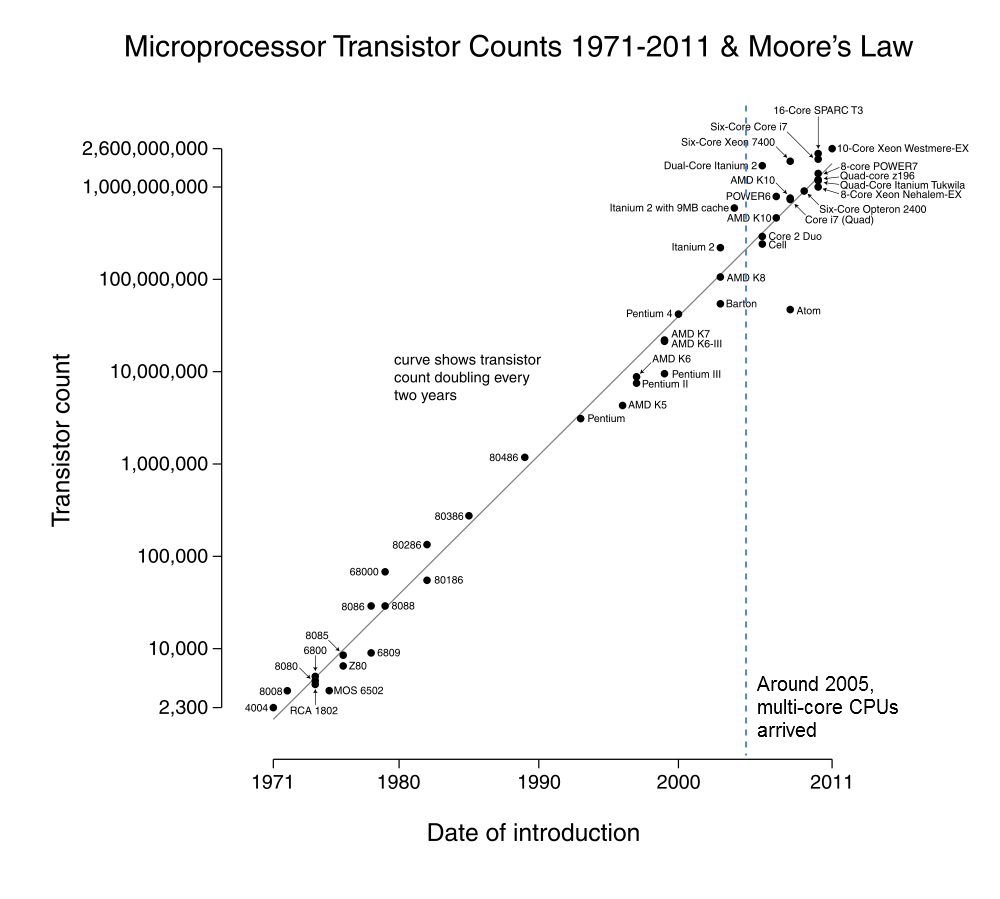
\includegraphics{MooresLaw.png}
\caption{Plot of CPU transistor counts against dates of introduction. Note the logarithmic vertical scale; the line corresponds to exponential growth with transistor count doubling every two years. This figure is from \href{http://en.wikipedia.org/wiki/File:Transistor\_Count\_and\_Moore\%27s\_Law\_-\_2011.svg}{Wikimedia Commons}.}\end{figure}

Therefore, CS students must learn principles of parallel computing to be prepared for careers that will require increasing understanding of how to take advantage of multi-core systems.


\section{Some pairs of terms}
\label{Introduction/Introduction:moore-s-law}\label{Introduction/Introduction:some-pairs-of-terms}\begin{description}
\item[{\index{parallelism|textbf}parallelism}] \leavevmode\phantomsection\label{Introduction/Introduction:term-parallelism}
multiple (computer) actions physically taking place at the same time

\end{description}
\begin{description}
\item[{\index{concurrency|textbf}concurrency}] \leavevmode\phantomsection\label{Introduction/Introduction:term-concurrency}
programming in order to take advantage of parallelism (or virtual parallelism)

\end{description}
\begin{quote}\begin{description}
\item[{Comments}] \leavevmode
Thus, parallelism takes place in hardware, whereas concurrency takes place in software. Operating systems must use concurrency, since they must manage multiple processes that are abstractly executing at the same time--and can physically execute at the same time, given parallel hardware (and a capable OS).

\end{description}\end{quote}
\begin{description}
\item[{\index{process|textbf}process}] \leavevmode\phantomsection\label{Introduction/Introduction:term-process}
the execution of a program

\end{description}
\begin{description}
\item[{\index{thread|textbf}thread}] \leavevmode\phantomsection\label{Introduction/Introduction:term-thread}
a sequence of execution within a program

\end{description}
\begin{quote}\begin{description}
\item[{Comments}] \leavevmode
Every process has at least one thread of execution, defined by that process's program counter. If there are multiple threads within a process, they share resources such as the process's memory allocation. This reduces the computational overhead for switching among threads (also called \emph{lightweight processes}), and enables efficient sharing of resources (e.g., communication through shared memory locations).

\end{description}\end{quote}
\begin{description}
\item[{\index{sequential programming|textbf}sequential programming}] \leavevmode\phantomsection\label{Introduction/Introduction:term-sequential-programming}
programming for a single core

\end{description}
\begin{description}
\item[{\index{concurrent programming|textbf}concurrent programming}] \leavevmode\phantomsection\label{Introduction/Introduction:term-concurrent-programming}
programming for multiple cores or multiple computers

\end{description}
\begin{quote}\begin{description}
\item[{Comments}] \leavevmode
CS students have primarily learned sequential programming in the past. These skills are still relevant, because concurrent programs ordinarily consist of sets of sequential programs intended for various cores or computers.

\end{description}\end{quote}
\begin{description}
\item[{\index{multi-core computing|textbf}multi-core computing}] \leavevmode\phantomsection\label{Introduction/Introduction:term-multi-core-computing}
computing with systems that provide multiple computational circuits per CPU package

\end{description}
\begin{description}
\item[{\index{distributed computing|textbf}distributed computing}] \leavevmode\phantomsection\label{Introduction/Introduction:term-distributed-computing}
computing with systems consisting of multiple computers connected by computer network(s)

\end{description}
\begin{quote}\begin{description}
\item[{Comments}] \leavevmode
Both of these types of computing may be present in the same system (as in our MistRider and Helios clusters).

\end{description}\end{quote}
\begin{description}
\item[{\index{data parallelism|textbf}data parallelism}] \leavevmode\phantomsection\label{Introduction/Introduction:term-data-parallelism}
the same processing is applied to multiple subsets of a large data set in parallel

\end{description}
\begin{description}
\item[{\index{task parallelism|textbf}task parallelism}] \leavevmode\phantomsection\label{Introduction/Introduction:term-task-parallelism}
different tasks or stages of a computation are performed in parallel

\end{description}
\begin{quote}\begin{description}
\item[{Comments}] \leavevmode
A telephone call center illustrates data parallelism: each incoming customer call (or outgoing telemarketer call) represents the services processing on different data. An assembly line (or computational pipeline) illustrates task parallelism: each stage is carried out by a different person (or processor), and all persons are working in parallel (but on different stages of different entities.)

\end{description}\end{quote}
\begin{description}
\item[{\index{shared memory multiprocessing|textbf}shared memory multiprocessing}] \leavevmode\phantomsection\label{Introduction/Introduction:term-shared-memory-multiprocessing}
e.g., multi-core system, and/or multiple CPU packages in a single computer, all sharing the same main memory

\end{description}
\begin{description}
\item[{\index{cluster|textbf}cluster}] \leavevmode\phantomsection\label{Introduction/Introduction:term-cluster}
multiple networked computers managed as a single resource and designed for working as a unit on large computational problems

\end{description}
\begin{description}
\item[{\index{grid computing|textbf}grid computing}] \leavevmode\phantomsection\label{Introduction/Introduction:term-grid-computing}
distributed systems at multiple locations, typically with separate management, coordinated for working on large-scale problems

\end{description}
\begin{description}
\item[{\index{cloud computing|textbf}cloud computing}] \leavevmode\phantomsection\label{Introduction/Introduction:term-cloud-computing}
computing services are accessed via networking on large, centrally managed clusters at data centers, typically at unknown remote locations

\end{description}
\begin{description}
\item[{\index{SETI@home|textbf}\href{mailto:SETI@home}{SETI@home}}] \leavevmode\phantomsection\label{Introduction/Introduction:term-seti-home}
another example of distributed computing

\end{description}
\begin{quote}\begin{description}
\item[{Comments}] \leavevmode
Although multi-core processors are driving the movement to introduce more parallelism in CS courses, distributed computing concepts also merit study. For example, Intel's recently announced 48-core chip for research behaves like a distributed system with regards to interactions between its cache memories.

\end{description}\end{quote}


\chapter{Parallel Speedup}
\label{ParallelSpeedup/ParallelSpeedup:parallel-speedup}\label{ParallelSpeedup/ParallelSpeedup::doc}

\section{Introduction}
\label{ParallelSpeedup/ParallelSpeedup:introduction}
The \emph{speedup} of a parallel algorithm \emph{over} a corresponding sequential algorithm is the ratio of the compute time for the sequential algorithm to the time for the parallel algorithm.  If the speedup factor is \emph{n}, then we say we have \emph{n-fold} speedup.  For example, if a sequential algorithm requires 10 min of compute time and a corresponding parallel algorithm requires 2 min, we say that there is 5-fold speedup.

The observed speedup depends on all implementation factors.  For example, more processors often leads to more speedup; also, if other programs are running on the processors at the same time as a program implementing a parallel algorithm, those other programs may reduce the speedup.  Even if a problem is embarrassingly parallel, one seldom actually obtains n-fold speedup when using n-fold processors.  There are a couple of explanations for this occurrence:
\begin{itemize}
\item {} 
There is often \emph{overhead} involved in a computation. For example, in the solar system computation, results need to be copied across the network upon every iteration. This communication is essential to the algorithm, yet the time spend on this communication does not directly compute more solutions to the n-body problem.
In general, communication costs are frequent contributors to overhead. The processing time to schedule and dispatch processes also leads to overhead.

\item {} 
\emph{trues} occur when a process must wait for another process to deliver computing resources. For example, after each computer in the solar system computation delivers the results of its iteration, it must wait to receive the updated values for other planets before beginning its next iteration.

\item {} 
Some parts of a computation may be inherently sequential. In the polar ice example, only the matrix computation was parallelized, and other parts gained in performance only because they were performed on faster hardware and software (on a single computer)

\end{itemize}

On rare occasions, using \emph{n} processors may lead to \emph{more} than an \emph{n}-fold speedup.  For example, if a computation involves a large data set that does not fit into the main memory of a single computer, but \emph{does} fit into the collective main memories of \emph{n} computers, and if an embarrassingly parallel implementation requires only proportional portions of the data, then the parallel computation involving \emph{n} computers may run more than \emph{n} times as fast because disk accesses can be replaced by main-memory accesses.

Replacing main-memory accesses by cache accesses could have a similar effect. Also, parallel pruning in a backtracking algorithm could make it possible for one process to avoid an unnecessary computation because of the prior work of another process.


\section{Amdahl's Law}
\label{ParallelSpeedup/ParallelSpeedup:amdahl-s-law}
\emph{Amdahl's Law} is a formula for estimating the maximum speedup from an algorithm that is part sequential and part parallel.  The search for \emph{2k}-digit primes illustrates this kind of problem: First, we create a list of all \emph{k}-digit primes, using a sequential sieve strategy; then we check \emph{2k}-digit random numbers in parallel until we find a prime.

The Amdahl's Law formula is
\begin{gather}
\begin{split}\textit{overall speedup} = \frac{1}{(1-P) +  \frac{P}{S}}\end{split}\notag
\end{gather}\begin{itemize}
\item {} 
P is the time proportion of the algorithm that can be parallelized.

\item {} 
S is the speedup factor for that portion of the algorithm due to parallelization.

\end{itemize}

For example, suppose that we use our strategy to search for primes using 4 processors, and that 90\% of the running time is spent checking 2k-digit random numbers for primality (after an initial 10\% of the running time computing a list of k-digit primes). Then P = .90 and S = 4 (for 4-fold speedup).  According to Amdahl's Law,
\begin{gather}
\begin{split}\textit{overall speedup} = \frac{1}{(1-0.90) + \frac{0.90}{4}} = \frac{0.10}{0.225} = 3.077\end{split}\notag
\end{gather}
This estimates that we will obtain about 3-fold speedup by using 4-fold parallelism.

\begin{notice}{note}{Note:}\begin{itemize}
\item {} 
Amdahl's Law computes the overall speedup, taking into account that the \emph{sequential} portion of the algorithm has no speedup, but the \emph{parallel} portion of the algorithm has speedup \emph{S}.

\item {} 
It may seem surprising that we obtain only 3-fold overall speedup when 90\% of the algorithm achieves 4-fold speedup. This is a lesson of Amdahl's Law: the \emph{non-parallelizable} portion of the algorithm has a disproportionate effect on the overall speedup.

\item {} 
A non-computational example may help explain this effect. Suppose that a team of four students is producing a report, together with an executive summary, where the main body of the report requires 8 hours to write, and the executive summary requires one hour to write and must have a single author (representing a sequential task). If only one person wrote the entire report, it would require 9 hours. But if the four students each write 1/4 of the body of the report (2 hours, in 4-fold parallelism), then one student writes the summary, then the elapsed time would be 3 hours---for a 3-fold overall speedup. The sequential portion of the task has a disproportionate effect because the other three students have nothing to do during that portion of the task.

\end{itemize}
\end{notice}

A short computation shows why Amdahl's Law is true.
\begin{itemize}
\item {} 
Let $T_s$ be the compute time without parallelism, and $T_p$ the compute time \emph{with} parallelism. Then, the speedup due to parallelism is

\end{itemize}
\begin{gather}
\begin{split}\textit{total speedup} = \frac{T_s}{T_p}\end{split}\notag
\end{gather}\begin{itemize}
\item {} 
The value P in Amdahl's Law is the proportion of $T_s$ that can be parallelized, a number between 0 and 1. Then, the proportion of $T_s$ that cannot be parallelized is 1-P.

\item {} 
This means that

\end{itemize}
\begin{gather}
\begin{split}T_p = \textit{time spent in unparallelizable code} + \textit{time spent in parallelizable code} = (1 - P) \times T_s + P \times \frac{T_s}{S}\end{split}\notag
\end{gather}\begin{itemize}
\item {} 
We conclude that

\end{itemize}
\begin{gather}
\begin{split}\textit{total speedup} = \frac{T_s}{T_p} = \frac{T_s}{(1 - P) \times T_s + P \times \frac{T_s}{S}} = \frac{1}{(1-P) +  \frac{P}{S}}\end{split}\notag
\end{gather}

\chapter{Some Options For Communication}
\label{OptionsForCommunication/OptionsForCommunication::doc}\label{OptionsForCommunication/OptionsForCommunication:some-options-for-communication}
In simple data parallelism, it may not be necessary for parallel computations to share data with each other during the executions of their programs. However, most other forms of concurrency require communication between parallel computations.  Here are three options for communicating between various processes/threads running in parallel.
\begin{enumerate}
\item {} 
\textbf{message passing} - communicating with basic operations \textbf{send} and \textbf{receive} to transmit information from one computation to another.

\item {} 
\textbf{shared memory} - communicating by reading and writing from local memory locations that are accessible by multiple computations

\item {} 
\textbf{distributed memory} - some parallel computing systems provide a service for sharing memory locations on a remote computer system, enabling non-local reads and writes to a memory location for communication.

\end{enumerate}
\begin{quote}\begin{description}
\item[{Comments}] \leavevmode
For distributed systems, message passing and distributed memory (if available) may be used. All three approaches may be used in concurrent programming in multi-core parallelism. However, shared (local) memory access typically offers an attractive speed advantage over message passing and remote distributed memory access.

\end{description}\end{quote}

When multiple processes or threads have both read and write access to a memory location, there is potential for a \textbf{race condition}, in which the correct behavior of the system depends on timing. (Example: filling a shared array, with algorithms for accessing and updating a variable \emph{nextindex}.)
\begin{itemize}
\item {} 
\textbf{resource} - a hardware or software entity that can be allocated to a process by an operating system

\end{itemize}
\begin{quote}\begin{description}
\item[{Comments}] \leavevmode
A memory location is an example of a (OS) resource; other examples are: files; open files; network connections; disks; GPUs; print queue entries. Race conditions may occur around the handling of any OS resource, not just memory locations.

\end{description}\end{quote}
\begin{itemize}
\item {} 
In the study of Operating Systems, \textbf{inter-process communication (IPC)} strategies are used to avoid problems such as race conditions. Message passing is an example of an IPC strategy. (Example: solving the array access problem with message passing.)

\item {} 
Message passing can be used to solve IPC problems in a distributed system. Other common IPC strategies (semaphores, monitors, etc.) are designed for a single (possibly multi-core) computer.

\end{itemize}


\chapter{Some issues in concurrency}
\label{ConcurrentIssue/ConcurrentIssue:some-issues-in-concurrency}\label{ConcurrentIssue/ConcurrentIssue::doc}
We will use the Hadoop implementation of map-reduce for clusters as a running example.

\textbf{Fault tolerance} is the capacity of a computing system to continue to satisfy its spec in the presence of faults (causes of error)
\begin{quote}\begin{description}
\item[{Comments}] \leavevmode
With more parallel computing components and more interactions between them, more faults become possible. Also, in large computations, the cost of restarting a computation may become greater. Thus, fault tolerance becomes more important and more challenging as one increases the use of parallelism. Systems (such as map-reduce) that automatically provide for fault tolerance help programmers of parallel systems become more productive.

\end{description}\end{quote}

\textbf{Mutually exclusive access to shared resources} means that at most one computation (process or thread) can access a resource (such as a shared memory location) at a time. This is one of the requirements for correct IPC.  One approach to mutually exclusive access is locking, in which a mechanism is provided for one computation to acquire a ``lock'' that only one computation may hold at any given time. A computation possessing the lock may then use that lock's resource without fear of interference by another process, then release the lock when done.
\begin{quote}\begin{description}
\item[{Comments}] \leavevmode
Designing computationally correct locking systems and using them correctly for IPC can often be quite tricky.

\end{description}\end{quote}

\textbf{Scheduling} means assigning computations (processes or threads) to processors (cores, distributed computers, etc.) according to time. For example, in map-reduce computing, we mapper processes are scheduled to particular cluster nodes having the necessary local data; they are rescheduled in the case of faults; reducers are scheduled at a later time.



\renewcommand{\indexname}{Index}
\printindex
\end{document}
